\documentclass[a4paper,12pt]{article}
\usepackage[utf8]{inputenc}
\usepackage{hyperref}
\usepackage{graphicx}
\usepackage{float}
\graphicspath{ {images/} }

\begin{document}

\begin{titlepage}

\newcommand{\HRule}{\rule{\linewidth}{0.5mm}} % Defines a new command for the horizontal lines, change thickness here

\center % Center everything on the page
 
%----------------------------------------------------------------------------------------
%-	HEADING SECTIONS
%----------------------------------------------------------------------------------------

\textsc{\LARGE University of Pretoria}\\[1.5cm]
\textsc{\Large COS 301 - Software Engineering}\\[0.5cm]
\textsc{\large The Savage Ru's}\\[0.5cm]

%----------------------------------------------------------------------------------------
%-	TITLE SECTION
%----------------------------------------------------------------------------------------

\HRule \\[0.4cm]
{ \huge \bfseries User Manual}\\ % Title of your document
\HRule \\[1.5cm]
 
%----------------------------------------------------------------------------------------
%-	AUTHOR SECTION
%----------------------------------------------------------------------------------------

\begin{minipage}{0.4\textwidth}
\begin{flushleft} \large
\emph{Author(s):}\\
Jodan \textsc{Alberts}\\ % Your name
Mark \textsc{Klingenberg}\\
Una \textsc{Rambani}\\
Ruan \textsc{Klinkert}\\
\end{flushleft}
\end{minipage}
~
\begin{minipage}{0.4\textwidth}
\begin{flushright} \large
\emph{Student number(s):} \\
14395283\\ % Student number
14020272\\
14004489\\
14022282\\

\end{flushright}

\end{minipage}\\[0.5cm]


%----------------------------------------------------------------------------------------
%-	DATE SECTION
%----------------------------------------------------------------------------------------

\centering
	
\includegraphics[width=80mm]{SavageRu.jpg}

{\large \today}\\[3cm] % Date, change the \today to a set date if you want to be precise

\centering
	\textsc{\LARGE Epi-Use labs project}\\[0.5cm]
	\textsc{\Large VizARD}\\[0.5cm]
	\textsc{\Large User Manual version 0.1}\\[0.5cm]
	
\includegraphics[width=\textwidth]{images/vizard.jpg}
%----------------------------------------------------------------------------------------

\vfill % Fill the rest of the page with whitespace

\end{titlepage}

\newpage

\tableofcontents

\newpage

\section{Introduction}

This is the user manual for the vizARD Augmented Reality application being developed for EPI-USE Labs by The Savage Ru's.

VizARD is a mobile application which will allow a user to take a picture of tabulated data and then view, automatically generated, 3D graphs of the data projected onto the document of which the image was taken.



%%--------------------------------------INSTALLATION  ----------------------------------------
\section{Installation}
To access the VizARD application one must first install it, currently this is done by getting the vizARD apk file, and installing it onto your android mobile phone (allow for the installation from unknown sources). In the future this app will be available through the Google play store.

%%-------------------------------------GETTING STARTED ----------------------------------------
\newpage

\section{Getting Started}
Once the app has been installed the user simply need to click on the application named VizARD, this will bring the user into a launching screen shown in figure 1.\\
\begin{figure}[H]
\centering
	
\includegraphics[width=50mm]{images/launch.png}
	\caption{launching screen \label{overflow}}
\end{figure}

Once the app has finished launching the user will be greated by the landing screen.
%%-------------------------------------LANDING SCREEN ----------------------------------------
\section{Landing Screen}
Once the app has completed loading it will then bring you to a screen that looks like figure 2, this screen shows what the camera is looking at as well as having two buttons currently, these are the capture data circle (Figure 3) that should be familiar to users of snapchat, as well as the View Previous graphs button (figure 4).

\begin{figure}[H]
\centering
	\includegraphics[width=50mm]{images/landing.png}
	\caption{landing screen \label{overflow}}
\end{figure}

\begin{figure}[H]
  \centering
  \begin{minipage}[b]{0.4\textwidth}
    
\includegraphics[width=50mm]{images/capture.png}
    \caption{Capture icon.}
  \end{minipage}
  \hfill
  \begin{minipage}[b]{0.4\textwidth}
    
\includegraphics[width=50mm]{images/graphRed.png}
    \caption{View Graphs.}
  \end{minipage}
\end{figure}



%%----------------------------------ON CAPTURE CLICK-----------------------------------------
\subsection{On Capture Circle click}
When a user clicks the capture data circle (figure 3) it will chose the table that is being viewed as the target for the 3D graph that will be generated, it will also send the image to a server to allow for optical character recognition of the data to make the graph, while this is occuring we plan to have some loading model to be placed on the target while the user waits. Once it has generated the graph the app moves to the display screen.

%%----------------------------DISPLAY GRAPH CLICK------------------------------------------------
\subsection{On View graphs click}
When a user clicks the View Graphs button (figure 4) currently nothing will happen as this section has not been implemented but we plan on it taking the user to screen shots of previous graphs they have decided to save. 
\newpage
%%----------------------------DISPLAY SCREEN------------------------------------------------
\section{Dispay Screen}
Once the app has completed generating the graph it will then bring you to a display screen that looks like figure 5, this screen shows the newly generated graph that has been mapped onto the target two buttons currently, these are the share graph button (Figure 6), as well as the edit graphs button (figure 6). We plan on implementing a save graph button that will also be here and will take a screen shot of the graph and save it. 

\begin{figure}[H]
\centering
	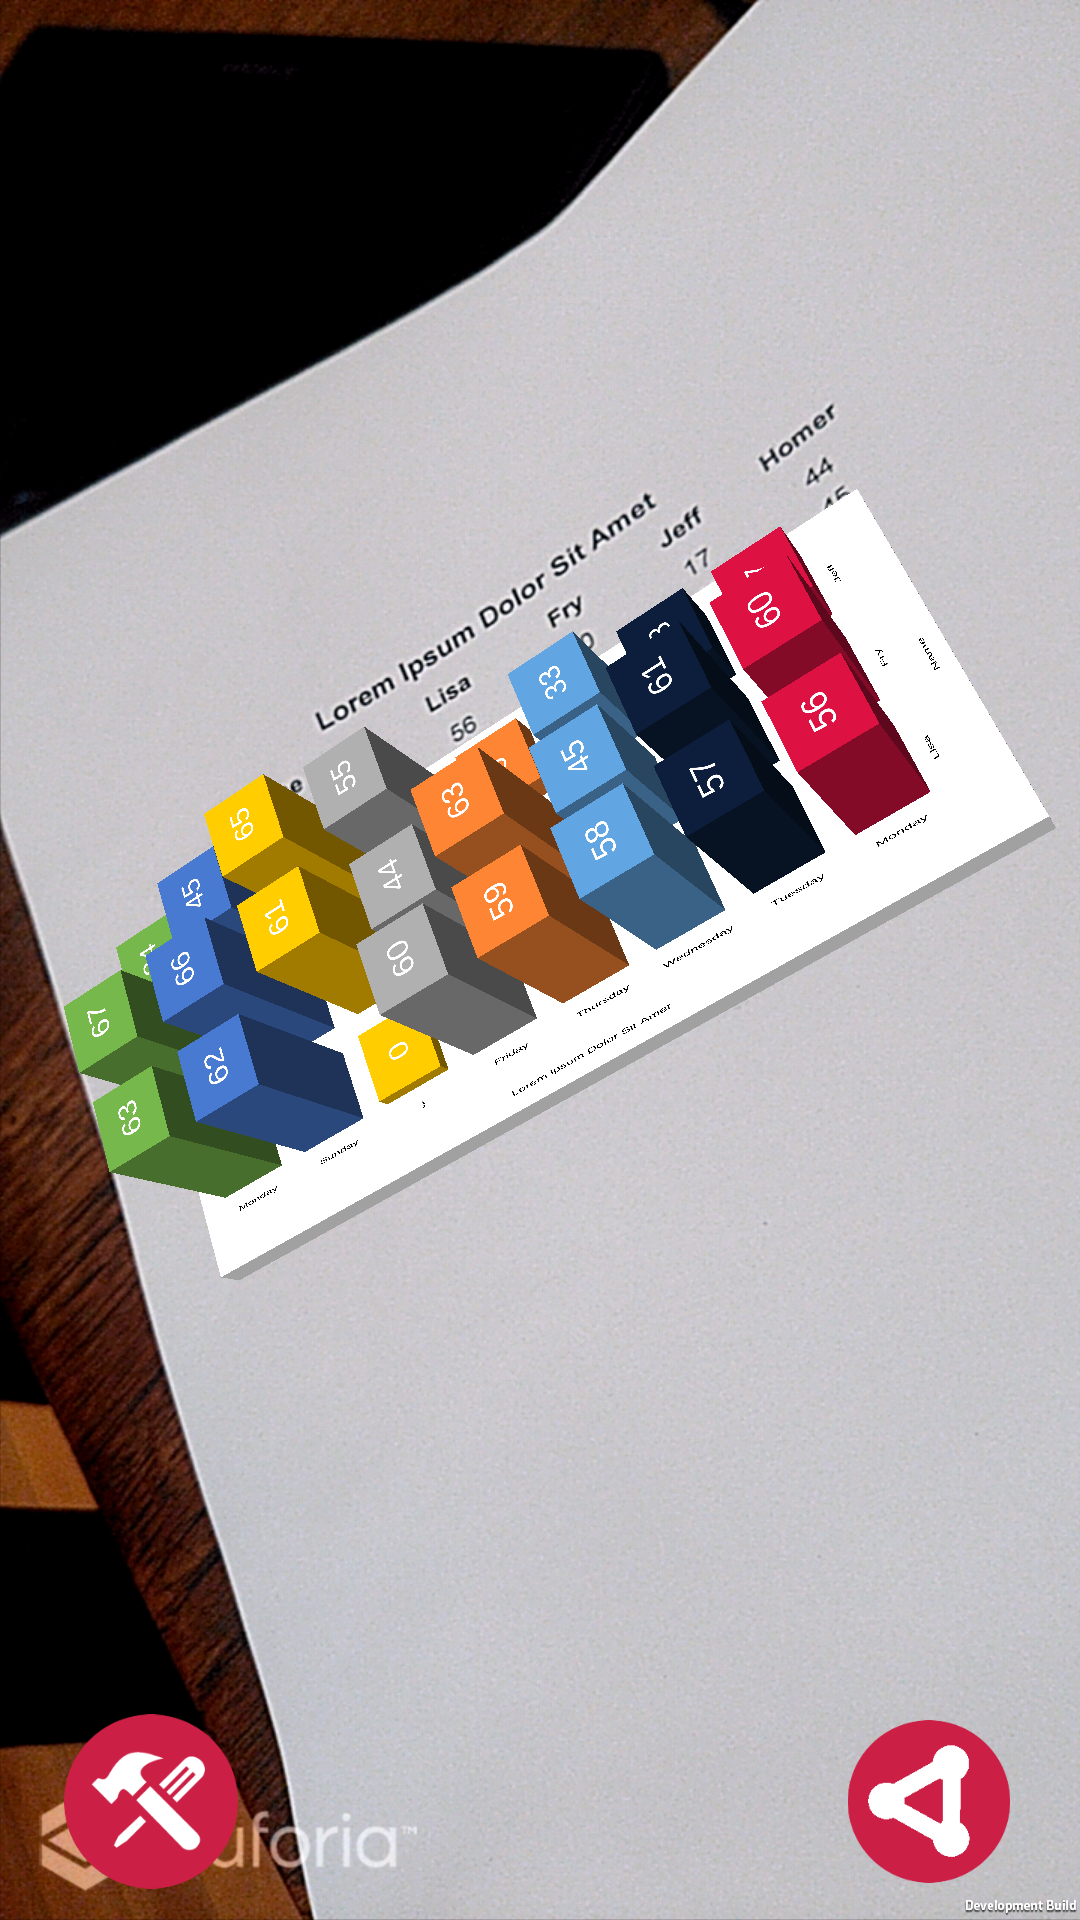
\includegraphics[width=8cm]{images/graph.png}
	\caption{display screen \label{overflow}}
\end{figure}

\begin{figure}[H]
  \centering
  \begin{minipage}[b]{0.4\textwidth}
    
\includegraphics[width=50mm]{images/editRed.png}
    \caption{Edit button}
  \end{minipage}
  \hfill
  \begin{minipage}[b]{0.4\textwidth}
    
\includegraphics[width=50mm]{images/shareRed.png}
    \caption{Share button}
  \end{minipage}
\end{figure}
\newpage
%------------------------on edit click------------------------------------
\subsection{On Edit Button click}
When the edit button is clicked a screen containing a form is showen, this form will allow the user to edit data and the graph. 
%-----------------------------form-----------------
\subsection{Form}
When the form is brought up from the edit button you see the following screen. 
\begin{figure}[H] 
\centering
    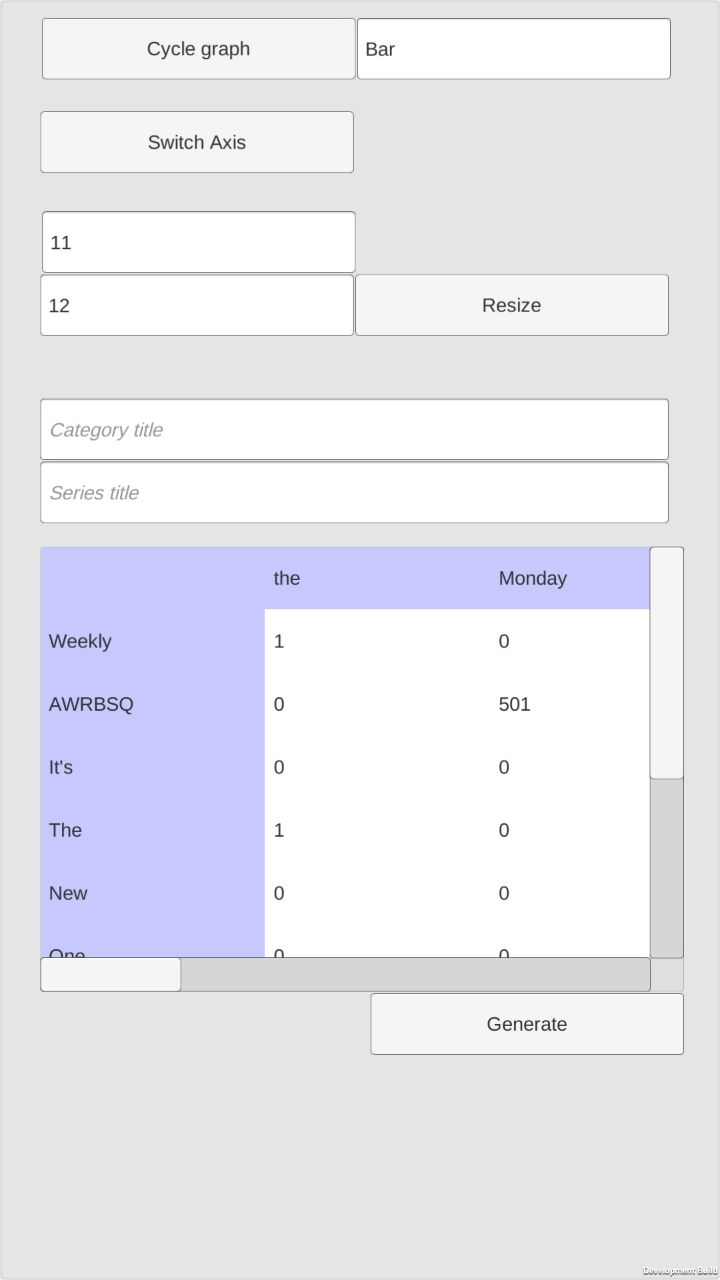
\includegraphics[width=85mm]{images/form.jpg}
    \caption{Edit form}
\end{figure}
The form contains a table that displays all the data that the OCR has read and generated the graph from, it also allows for the switching of axis, when the switch axis button is clicked, and you can cycle through graph type by pressing the "Cycle graph" button. 

%------------------------on Share click------------------------------------

\subsection{On Share Button Click}
The share button has not been implemented but once it has when a user clicks it the app will take a screen capture of the graph and open up genral sharing option such as share to facebook or whatsapp.

\end{document}